\documentclass{article}
\usepackage{graphicx} % Required for inserting images
\usepackage{hyperref} 
\usepackage[utf8]{inputenc} % Allow Unicode characters
\usepackage{amsmath} 
\usepackage{gensymb} % For \degree symbol
\usepackage{comment}
\title{Handbook of QPT's LabView}
\author{Yujie Sun}
\date{April 2025}

\begin{document}

\maketitle

\begin{comment}

\section{Beam Expander}
In order to expand the beam diameter from 2mm to 40mm and make it as homogeneous as possible, two diffusers were used. The coupling efficiency from the SM fiber to the cell is around $25\%$. The polarization is along the z-axis, which is parallel to the leading magnetic field. 
\begin{figure}[htbp]
    \centering
    \includegraphics[width=0.7\linewidth]{fig/Beam Profile Setup.png}
    \caption{Beam Expander}
    \label{fig:enter-label}
\end{figure}

\section{Vector Vortex Beam}
Design the setup to generate a vector vortex beam with a net vortex, as shown in Fig.~\ref{fig: VVB setup}.\\

\begin{figure}[htbp]
    \centering
    \includegraphics[width=0.9\linewidth]{fig/VVB Setup.png}
    \caption{Setup for generating the Vector Vortex Beam with a net vortex}
    \label{fig: VVB setup}
\end{figure}

Test successfully the spacial polarization of the VVB with a linear polarizer. However, it did not test the vortex number because it's very hard to overlap the vortex center perfectly when creating the vector beams.
\begin{figure}[htbp]
    \centering
    \includegraphics[width=0.65\linewidth]{fig/VVB Pol res.png}
    \caption{Polarization test of the VVB}
    \label{fig: VVB result}
\end{figure}

The space light modulation (SLM) is from Holoeye, the controlling software can be obtained from Link \url{https://holoeye.com/downloads/}. There are some standard phase holograms in the software, or it's also possible to use homemade phase holograms. The phase hologram is a gray picture; in general, the resolution is 0-255. If it is 0, it means that SLM does not add any phase on the beam, as for 255, SLM will add 2pi phase on the beam, as shown in the Fig.~\ref{fig: hologram}.
\begin{figure}[htbp]
    \centering
    \includegraphics[width=0.5\linewidth]{fig/Vortex=1.png}
    \caption{Homemade phase holograms with Vortex = 1}
    \label{fig: hologram}
\end{figure}
\begin{figure}[htbp]
    \centering
    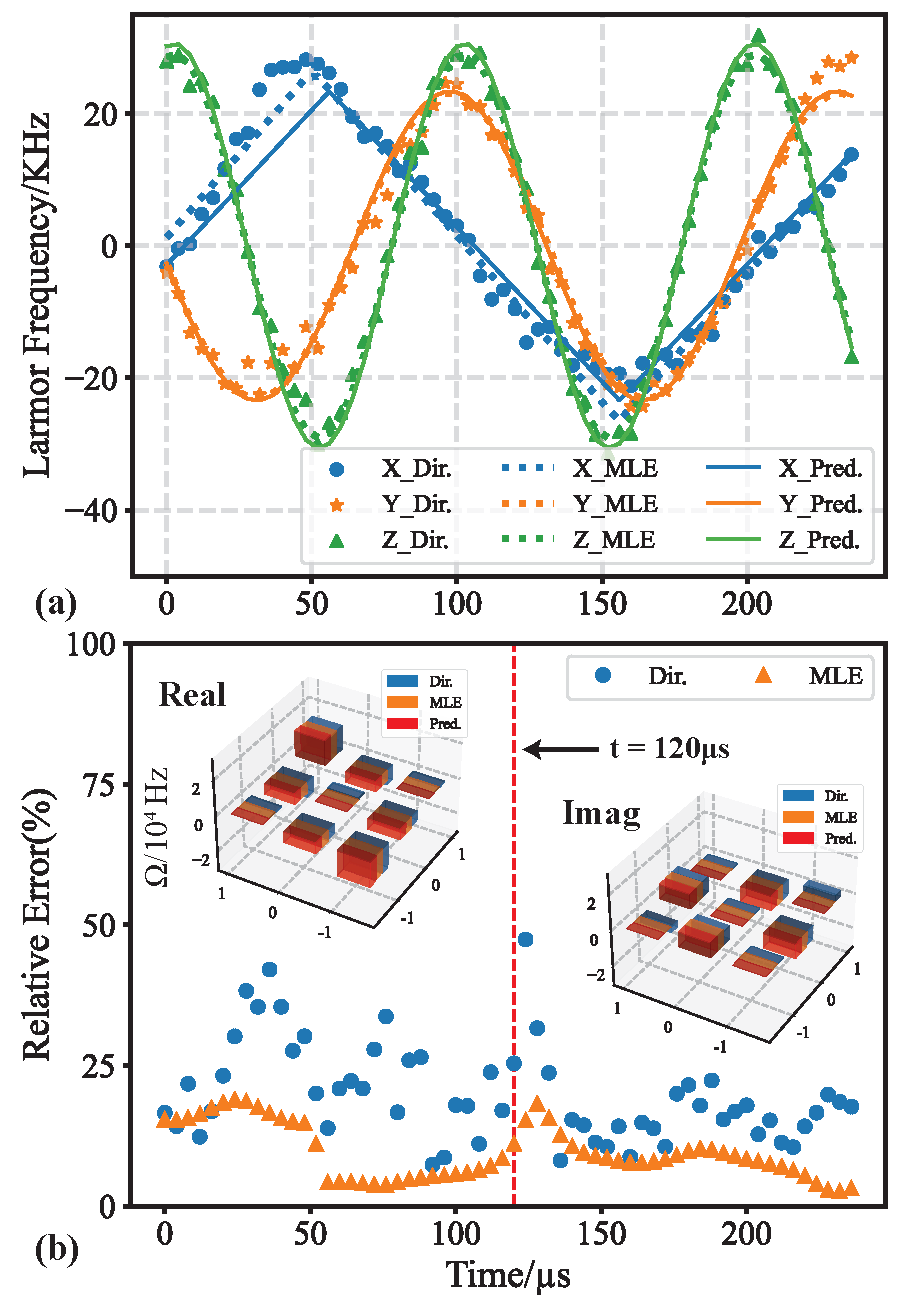
\includegraphics[width=0.5\linewidth]{fig/NewHt.pdf}
    \caption{Reconstruction of the time-dependent Hamiltonian}
    \label{fig: VVB result}
\end{figure}
\end{comment}
\section{Introduction}
Realize the reconstruction of the time-dependent Liouvillian. The main experimental program is shown in the next section, here is the result on the time-dependent Liouvillian. The detailed results will be published in the paper. Here is the link: \url{https://arxiv.org/abs/2508.19634}.   

\section{Experimental program in Labview}
\subsection{Original Timing Sequence}
The heart of the experimental program in Labview is precise timing. We used an NI data acquisition card named NI-PCI 6259 to provide robust timing, digital output, and analog input for the whole experiment. 
\begin{figure}[htbp]
    \centering
    \includegraphics[width=1\linewidth]{fig/Timing.png}
    \caption{The front Panel of the timing sequence in the Example file}
    \label{fig:timing}
\end{figure}

As shown in Fig.~\ref{fig:timing}, the numbers in odd positions represent the duration time of the high digital level. Otherwise, the numbers in the even positions represent the duration time of the low digital level. As you can see, there are four 1000 in the Timing 0, which means that the signal is a 1000us high, 1000us low,1000us high, 1000us low signal (red 
 line).  Moreover, the resolution of the timing Sequence can be changed; the minimum timing resolution is 50ns, i.e., 20MHz. But we just set 10MHz as the digital clock in the experiment, which is the Sample Freqeuncy shown in the blue box of Fig.~\ref{fig:timing}. The total timing period is dependent on:
 \begin{equation}
     Period = \frac{Sample\; Numbers}{Sample \;Frequency}=\frac{20M}{10MHz} = 2s
 \end{equation}
 \begin{figure}[htbp]
    \centering
    \includegraphics[width=1\linewidth]{fig/Example for Timing sequence.png}
    \caption{The rear panel of the timing sequence in the Example file. Blue Box: the transformation file from the experimental timing sequence data to the machine data. Red box: The real timing pulse will be generated, according to the machine data from the blue box file.}
    \label{fig:rear panel}
\end{figure}
\begin{figure}[htbp]
    \centering
    \includegraphics[width=1\linewidth]{fig/TimeSequence_creation.png}
    \caption{Time Sequence creation. The digital clock is the basic frequency (red line). According to this basic frequency, the digital output (blue line) can be precisely created. All digital triggers of the instrument in the experiment will follow the digital output signal. The analog clock (yellow line) also follows the digital clock by counting the numbers of the TTL, which can control the timing of the analog signal (green line).}
    \label{fig:time sequence}
\end{figure}
The corresponding rear panel of the timing sequence is shown in Fig. \ref{fig:rear panel}. The blue box represents the transformation file from the experimental timing data to the machine timing data, while the red box represents the pulse generation file. Figure \ref{fig:time sequence} shows the most important part of how to create the analog signal and digital signal in the NI device, which is exactly the pulse generation file shown in Fig.~\ref{fig:rear panel}. The digital clock is the basic frequency (red line), which is the digital sample frequency (10MHz). All digital output (blue line) will follow this basic frequency to get the precise time of the experiment and control the preset timing sequence. Then, all digital triggers of the instrument in the experiment will follow the digital output signal and be active at the corresponding time. Moreover, the analog clock (yellow line) also synchronously follows the digital clock by counting the numbers of the TTL, which will be used to generate and obtain the analog signal. In our experiment, it will be used to obtain the probe beam power (green line) before entering the shield to get the global scaling factor. If you want to get some detailed tutorials, you can see the documents on the NI website \url{https://www.ni.com/en/support/documentation/supplemental/06/timing-and-synchronization-features-of-ni-daqmx.html?srsltid=AfmBOop9MO7PBRj0Iug0jmJ8uzTod82ty7YdeHwMMM00kIJsP22Vu4ZO}
\subsection{Introduction of the user interface}
\subsubsection{Design the sequence\label{subsubsec:Qst}}
The LabVIEW control software of the experiment is shown in Fig~\ref{fig:pathway}. The addons used in the experiment are Keithley, Zurich, and NI Daq, which are saved in the file "Addons". The corresponding configuration can be found in the file "Config Files". The main entrance of the program is in the file "Main", and the user interface of the basic version and the newest version is "main control v1" and "main control YJtoy V6", respectively. Some functions used in the "main control YJtoy V6" can be found in the file "YJtoy."
\begin{figure}[htbp]
    \centering
    \includegraphics[width=0.8\linewidth]{fig/Project.png}
    \caption{The main pathway of the software and introduction.}
    \label{fig:pathway}
\end{figure}
\begin{figure}[htbp]
    \centering
    \includegraphics[width=0.9\linewidth]{fig/State preparation.png}
    \caption{The user interface of the sequence design.}
    \label{fig:UI}
\end{figure}
The user interface of the sequence design of the experimental software is shown in fig.~\ref{fig:UI}, which displays the detailed layout of the function mode named "Design the sequence", i.e.,
\begin{itemize}
    \item 0. Function Zone. 
    
    Function Zone is in the top menu, and you can double-click it to select the different modes for the corresponding situation.
    \item 1. Pump Zone

    To make the thermal atomic state as close to the pure state as possible, it's necessary to add the pump and repump beams simultaneously. The enumeration control button named "pumping" is used to select the leading magnetic field during the pumping stage. And the buttons named "Add pumping" and "Rest Sequence" are used to add a pumping sequence automatically and reset the total sequence. Generally, you need to press the button "Add pumping" first when you want to experiment. But if you just want to create some special timing sequence, e.g., process sequence in quantum process tomography, the button can be ignored.   
    
    \item 2. Manipulation Zone

    To rapidly design any interaction between the magnetic field and the atomic states, some special buttons are placed in the Manipulation Zone. The "X pi" button means that it will create a magnetic field along the x-axis pulse, and the corresponding pulse duration is the Larmor period required for an atom to rotate through the $\pi$ phase. The other buttons, like "Y/Z pi" have the same influence. It should be noted that the "AOC" button is equal to the "X pi/4" button. Moreover, if you want to add other channels you create or something else, you can input the duration in the "Time" control and the channel name in the "Channel"  control. Then press the "Add pulse" button to add the time sequence. Finally, suppose you want to add two or more channels simultaneously. In that case, you can input them in the "Physical channels" control, input the duration in the "Time" control, and add them by pressing the "Add pulse advanced" button.  
    
    \item 3. Timing Sequence Display Zone

    This zone is to display the pulse sequence of each channel during the application. It should be noted that there are 23 channels in the NI DAQ, which have been occupied by 18 actions and have 5 void channels left to use. If you want to check the meaning of each channel, you can see them in the Function Zone "Presets" or you can check the map of the channels and actions in the back panel (see fig.~\ref{fig:DAQ-preset}).
    
    \item 4. Initialization and Process Zone

    If you are doing the quantum process tomography experiment, after creating the sequence that you want, you can save it as an initial state file or a process file. Noted that the sequence might not be seen in the timing sequence display zone when you create a short process pulse. You need to adjust the scale of the x-axis of the LabVIEW oscilloscope to get it. 
    
    \item 5. Single save and Run Zone

    If you are doing the Freedom-induced decay or quantum state tomography, you can save them and run them in this Zone.
    
    \item 6. Batch save Zone

    If you want to produce a batch of time sequences, you can set the start time in the "Start time" control, the single period time in the "Period" control, and the period number in the "Period number" control. For example, when the "Start time" = 10, "Period" = 20, "Period number" = 30, it means that 30 timing sequence files will be created, the action caused by the "Channel" control will last  10 us in the first file, the action of the second file will last 10+20=30 us, the third one last 10 + 20*2 = 50 us, and so on. The final one is  10 + 20*29 = 590 us. Each channel's action duration can be checked in the presented pulses of Fig.~\ref{fig:DAQ-preset} or "Time" control in the Manipulation Zone.
\end{itemize}

\begin{figure}[htbp]
    \centering
    \includegraphics[width=0.8\linewidth]{fig/DAQ_Preset.png}
    \caption{The DAQ preset of the back panel}
    \label{fig:DAQ-preset}
\end{figure}

\subsubsection{Design QPT}
\begin{figure}[htbp]
    \centering
    \includegraphics[width=1\linewidth]{fig/Process Selection.png}
    \caption{The user interface of the quantum process tomography design}
    \label{fig:process selection}
\end{figure}
In the section \ref{subsubsec:Qst}, we know how to save the initial state and process file, but to run the quantum process tomography automatically, in this section we will introduce how to save the total quantum process tomography files.

As shown in fig.~\ref{fig:process selection}, the user interface of the QPT design can be split into five parts:
\begin{itemize}
    \item 0. State/Process set

    In this part, some initial states/ process sequences can be selected, which are shown by the blue box. If you don't see any initial state/process file, you can click the "State Update"/"Process Update" button to refresh this part. If you still don't see the files, you should check whether you saved these files in the previous phase, i.e., Design the sequence.  
    
    \item 1. State/Process Display

    In this zone, you can check the time sequence of the State/Process. For example, the time sequence of the file named "initial state 02.ini" is being displayed in the State Display zone of Fig.~\ref{fig:process selection}.      
    
    \item 2. Operation

    In this zone, you could choose the  State/Process time sequence files and put them into the queue used in the QPT experiment. The button "Choose Initial State" will add the file, which was shown in "State set", into the List "The Chosen States". The button "Delete Initial State" will delete the file shown in "State set" if there is a true file. The "Show States List" button will display all files in "The Chosen States". And the button "Clear States list" will delete all files in "The Chosen States". Similarly, there are four buttons which has the same operation but for operating the Process sequence files.  
    
    \item 3. Selected State/Process

    This Zone shows the atomic States/Process files that will be used in the experiment. If you want to change the files, you should use the previous operation to modify them.
    
    \item 4. Save and Run

    Once you ensure the State/Process, you can use the button "Save QPT" to automatically create the files that will be used exactly in the experiment. And the button "Run QPT" will start the experiment. 
    
\end{itemize}


\subsubsection{Run Single FID}

\begin{figure}[htbp]
    \centering
    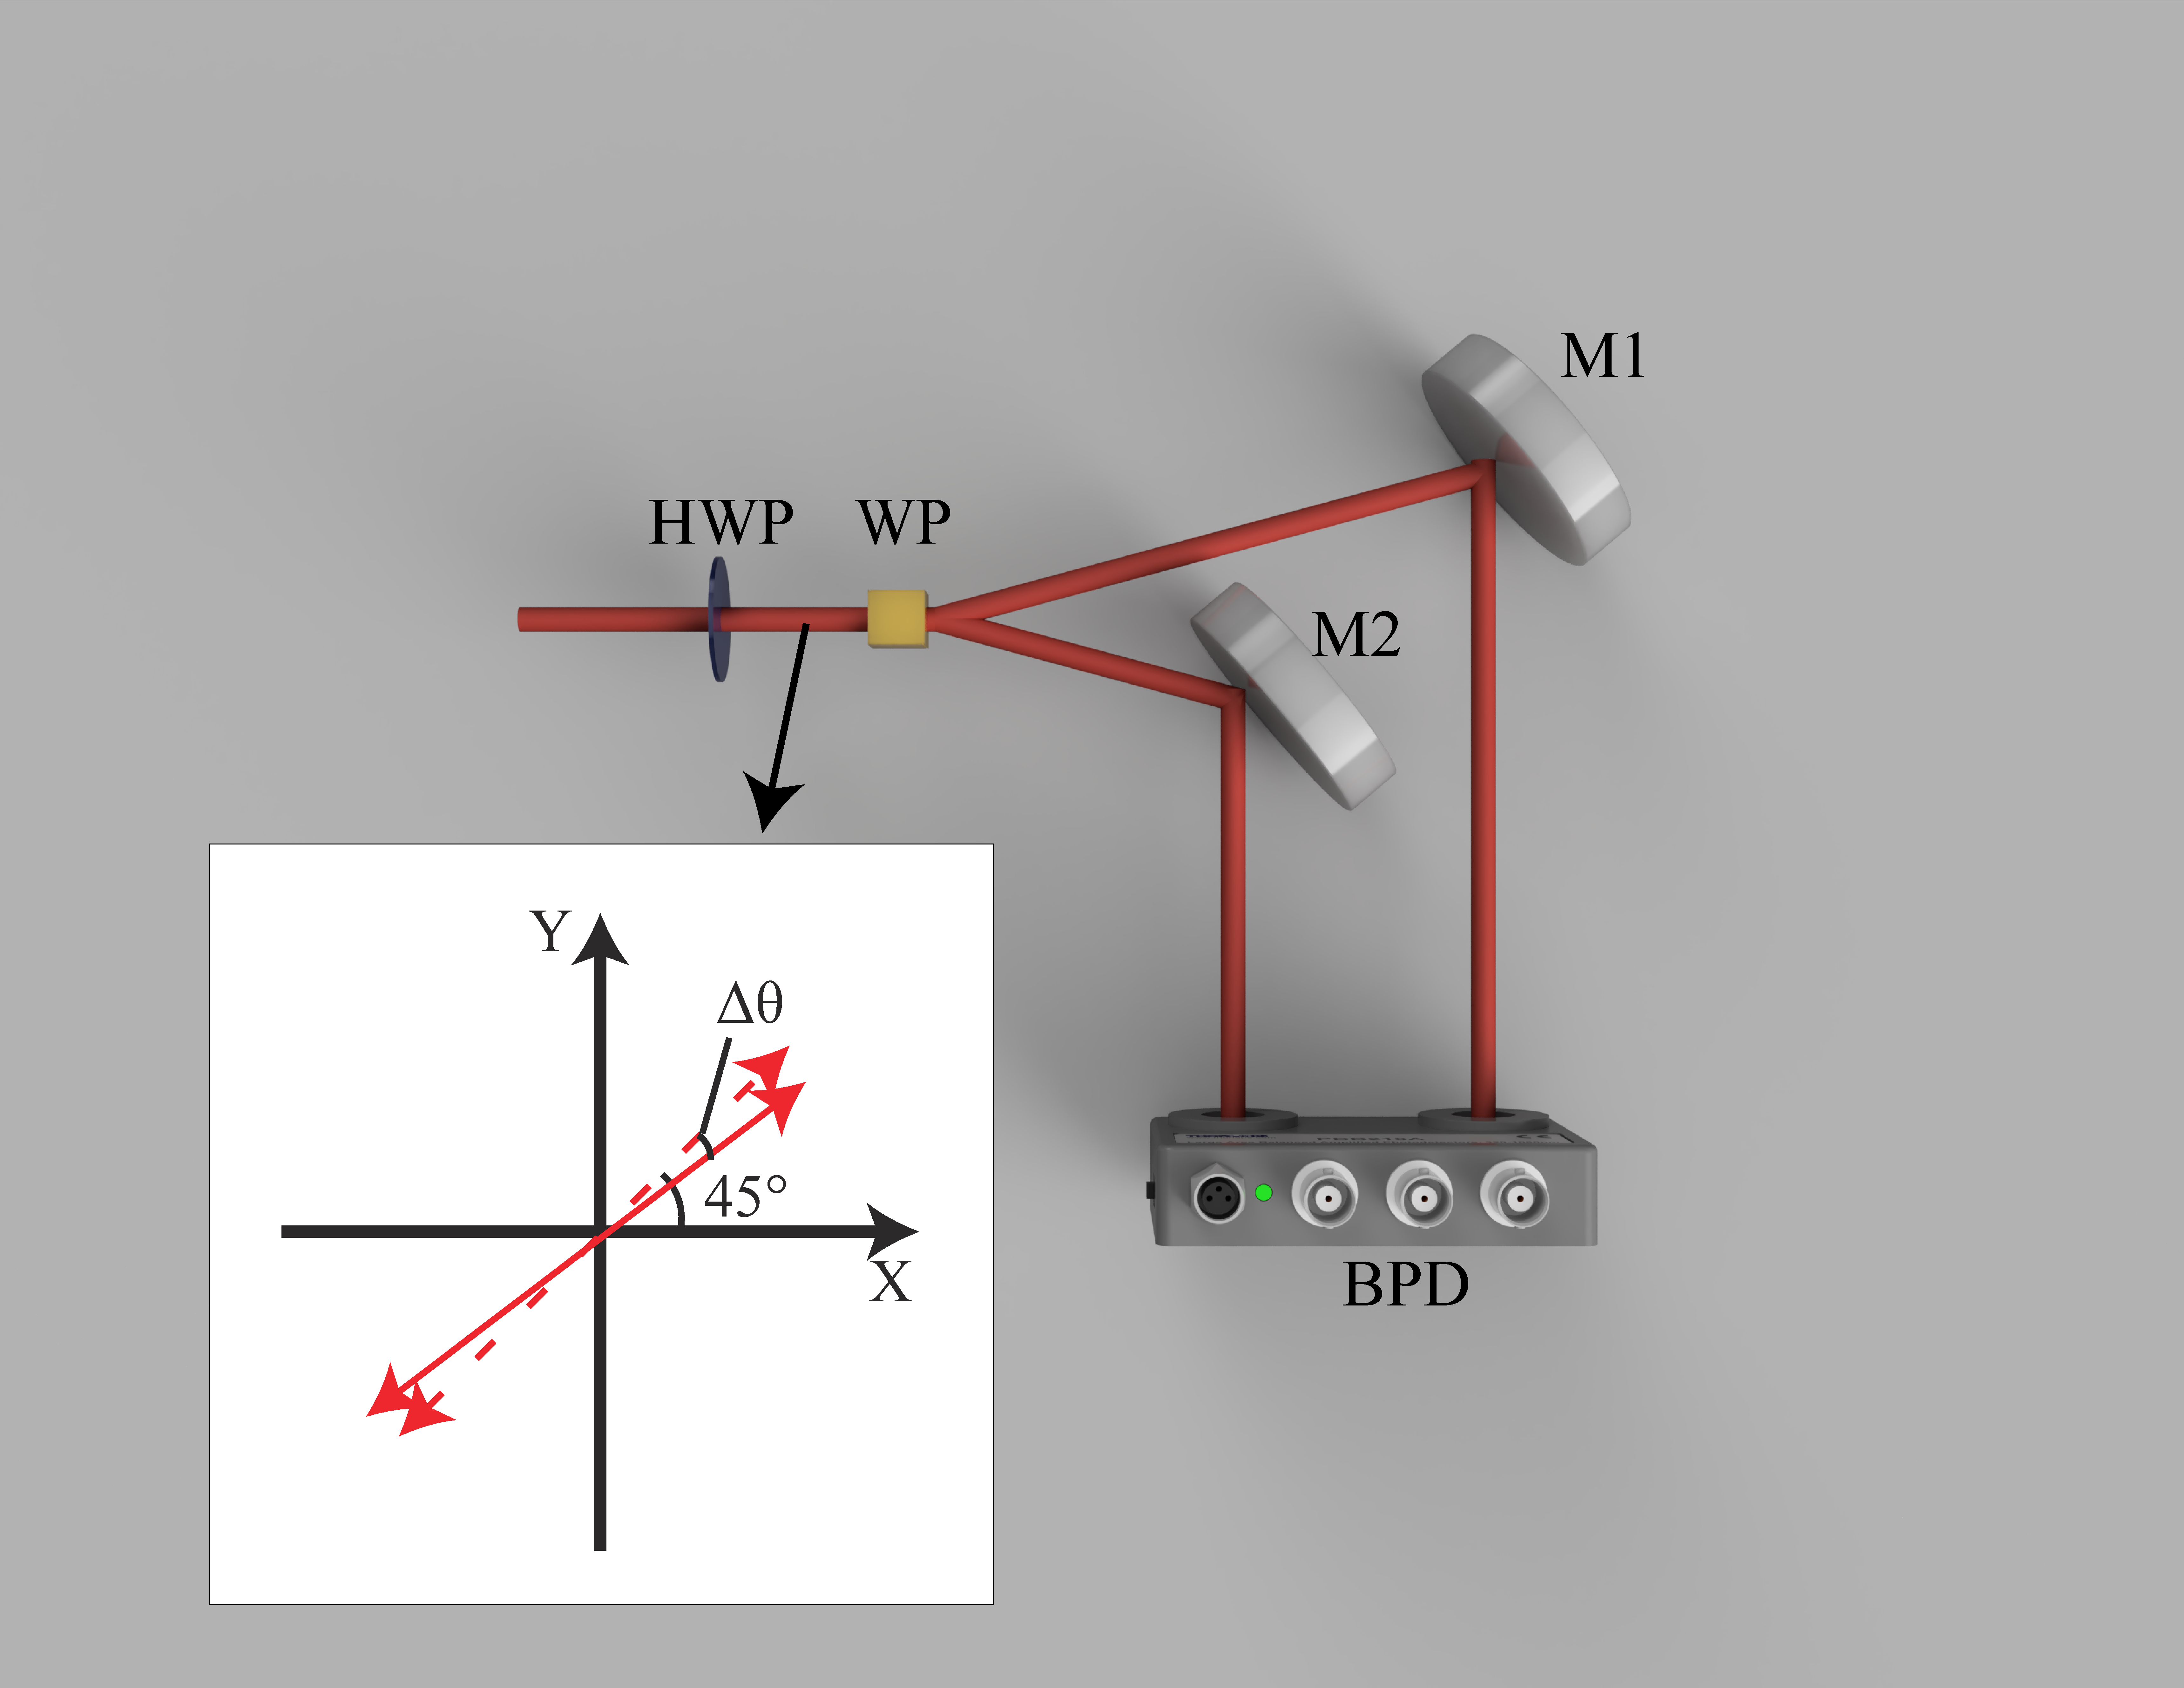
\includegraphics[width=0.9\linewidth]{fig/Rotation.pdf}
    \caption{The schematic diagram of the balanced detection.}
    \label{fig:rotation}
\end{figure}

The Free induction decay (FID) signal represents the time-domain response of spins after they have been perturbed by a pulse. In our experiment, there will be a leading magnetic field added on the z-axis during the probing, and the polarization of the probe beam is along the y-axis. When the probe beam crosses the atoms, the polarization will be changed by the polarized atoms. So, the target of the section named "Run Single FID" here is to record the change of the polarization of the probe beam. As shown in Fig.~\ref{fig:single FID}, there are some zones to measure and check the FID signal, and we will introduce them one by one.

Before introducing the FID signal, we need to have some prior knowledge of balanced detection. As shown in Fig.~\ref{fig:rotation}, first, the differential intensity between the x-axis and y-axis should be calibrated to 0 by using a half-wave plate, which means that the angle between the linear polarization and the x-axis should be $45^{\circ}$ before the beam goes through the Wollaston prism. Second, if there is a small change in the atomic system, it will affect the polarization angle of the probe beam, which we assume it is a slightly different angle $\Delta\theta$. Then, the new different intensity $\Delta I$ is:
\begin{equation}
    \begin{aligned}
        \Delta I &= I_{Y}-I_{X}\\
        &=I\sin^2(\frac{\pi}{4}+\Delta\theta)-I\cos^2(\frac{\pi}{4}+\Delta \theta)\\
        &=2I\Delta\theta+O[(\Delta\theta)^3],
        \label{eq:Rotation Relationship}
    \end{aligned}
\end{equation}
where $I$ is the total intensity of the probe beam. Ignoring the higher-order affection of $\Delta\theta$, $\Delta I = 2I\times\Delta \theta$.

\begin{figure}[htbp]
    \centering
    \includegraphics[width=1\linewidth]{fig/FID signal.png}
    \caption{The user interface of the free induction decay.}
    \label{fig:single FID}
\end{figure}

\begin{itemize}
    \item Total Intensity


    The total intensity of the probe beam can be checked in this zone. In general, the total intensity will be largely absorbed at the beginning, due to the pure state of the initial state. As the atomic state is gradually destroyed, the interaction between the probe beam and the atoms will decrease. Thus, the total intensity detected by the PD will increase and reach a balance stage. The shape of the total intensity is shown in the Total Intensity Zone of Fig.~\ref{fig:single FID}.       
    \item Differential Intensity


    The intensity difference of the probe beam with polarization along the x-axis and y-axis can be checked in this zone. In order to improve the Signal-to-Noise Ratio, the probe beam is modulated and demodulated by the Lock-in Amplifier. Thus, we will get two intensity difference signals, i.e., in-phase component and quadrature component. Noted that one of the components of the intensity difference signals should be set at a maximum by changing the phase of the reference in the Zurich software. In the Differential Intensity Zone of Fig. \ref{fig:single FID}, we make the red signal a maximum by setting the reference phase as $102\degree$ in the Zurich software. 

    \item Rotation Angle

    The rotation angle representing the intensity of light-atom interaction can be checked in this zone. According to Eq.~\eqref{eq:Rotation Relationship}, the rotation angle complies with $\Delta\theta=\frac{\Delta I}{2I}$. The total intensity comes from the Total Intensity Zone, and the intensity difference comes from the Differential Intensity Zone. Noted that there are two signals in the Differential Intensity Zone, i.e., in-phase and quadrature signals, we should choose the signal with the highest intensity by switching the button of "Signal in X or Y".
    
    \item Fitting

    The parameters of the FID signal of the Rotation Angle will be shown. Two fitting models could be chosen. The first is cosine type, that is, $A\cos\left(wt+q \right)e^{-g_1t}+C$, and the second is full type, i.e., $A\cos\left(wt+q \right)e^{-g_1t}+Be^{-g_2t}+C$.  
     
    \item Rotation Spectrum

    In this Zone, the frequency spectrum of the in-phase and quadrature signals will be checked. In the experiment, the Larmor frequency caused by the leading magnetic field is around 1 kHz.
    
    \item Polarimeter

    The Polarimeter is used to check the initial calibration of the system by summing all rotation angles. In the case of the orientation atomic state along the x-axis by a circularly polarized beam, the sum of the rotation angle should be close to 0. In practice, the range of the Polarimeter is between -3 and 3. If it's not in this range, we should slightly modify the angle of the Half Wave Plate in the balanced detection part, as shown in Fig. \ref{fig:rotation}.
    
\end{itemize}

\subsubsection{Run QST and QPT}
\begin{figure}[htbp]
    \centering
    \includegraphics[width=0.95\textwidth]{fig/QST_signal.png}
    \vspace{0.5cm}
    \includegraphics[width=0.95\textwidth]{fig/QPT_signal.png}
    \caption{The user interface of the QST (top) and QPT (bottom). Here, because the user interfaces of QST and QPT are very similar, I just use the QST picture to represent both QST and QPT. }
    \label{fig:QST and QPT}
\end{figure}
Since Quantum State Tomography and Quantum Process Tomography are both based on the FID signal measurements, their user interfaces are very similar to the FID's, as shown in Fig.\ref{fig:QST and QPT}. There are the total intensity, differential signal, the average rotation angle for the measurement, and the rotation signal's spectrum, which are the same as the FID's. Noted that the data can be saved as CYCLOPS/raw form in QST, but in the QPT case, the data can only be saved as CYCLOPS form, even if you press the "raw data 2" button (I don't remember clearly, but you can check the code). 
\subsection{Introduction of the experimental operation about the QPT}
\subsubsection{Principle of the Sequential Creation}
\begin{figure}[htbp]
    \centering
    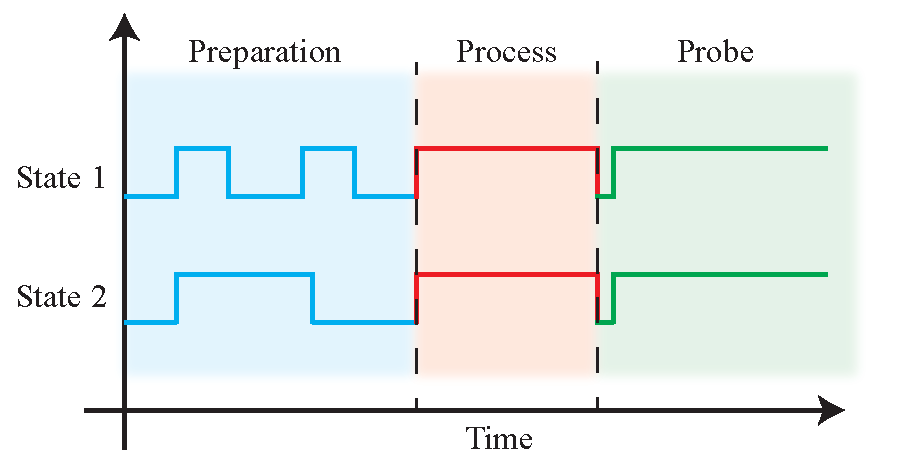
\includegraphics[width=0.9\linewidth]{fig/TimeSeq.pdf}
    \caption{The schematic diagram of the QPT time sequence}
    \label{fig: QPT time seq}
\end{figure}
To characterize precisely the evolution of the environment, we create 16 initial states, including 15 initial states for probing and 1 circular state for getting the local scaling factor of the quantum state tomography, to reconstruct the Liouville operator. The main schematic diagram of the QPT experimental time sequence is shown in Fig. \ref{fig: QPT time seq}. It should be noted that different initial states may have different time sequences to create, which means the preparation time of the different states may be different. To avoid such things from disturbing the experiment, the program has added automatically a delay time to ensure that the different states have the same preparation time. Then, these states will be sent into the same process of interest and reconstructed in the probe stage eventually. 

\subsubsection{The experimental files of QPT}
The QPT measurement time sequence files are saved in Link:\url{Labview/QST/Config_Files/Config_Ver_2/process}. As shown in Fig. \ref{fig: time sequence files}, three files can be accessed, including the initial states file, the process file, and the temporary state files combining the preparation, process and time sequence of the quantum state tomography. Note that the temporary state files are the actual time sequence files, which will be automatically loaded by the software when pressing the "run QPT" button.      

\begin{figure}[htbp]
    \centering
    \includegraphics[width=0.9\linewidth]{fig/QPT.pdf}
    \caption{The time sequence files}
    \label{fig: time sequence files}
\end{figure}

\subsubsection{The automatic creation of the process}
For a specific process, you can input it by hand, which is the same operation as the initial state creation. However, if you want to create a batch of the process, like 0us,2us,4us,..., until to 100us, you can set the start time as 0us, period time as 2us, and Period number as 51. Then, press the "Save multi-process" botton and these time sequences of the processes will be automatically saved in the process file. Note that before you set these parameters, the first thing is that you should choose which channel will be used to create the process. For example, if you want to change the time duration of channel X, you should click the "Channel", and choose "Pulse X", as shown in Fig.\ref{fig:UI}.

\subsubsection{Arbitrary process creation}

\begin{figure}[htbp]
    \centering
    \includegraphics[width=0.9\linewidth]{fig/Arb Gen.png}
    \caption{The schematic diagram of the generation of the arbitrary signal}
    \label{fig: arbitrary signal generation}
\end{figure}

Before discussing the specific operation, we must understand how to create an arbitrary process at the physical level in the experiment. As shown in Fig.\ref{fig: arbitrary signal generation}, the current sources of the pulses X, Y, and Z are from three independent Arbitrary Function generators, which could generate any designed signal. The signals will then be sent through the Pulse Amplifier, which not only amplifies the signal current but also determines whether the signal will be sent to the system. The time sequence of the Function Generator and Pulse Amplifier is decided by the NI-DAQ, where Port 1/line 5 will trigger these three Function Generators to start working simultaneously, and Port 1/line 6, Port 1/line 7, and Port 2/line 1 control the Switch of the pulse X, Y, and Z, respectively. In practice, the opening order of the action from these three signals is as follows:
\begin{enumerate}
    \item First, Port 1/line 6, Port 1/line 7, and Port 2/line 1 will switch on the channels of these three Pulse Amplifiers 10 us in advance.
    \item Second, Port 1/line 5 will trigger these Function Generators to start working simultaneously. 
    \item Third, these four lines of the NI DAQ will continue for a designated time.
    \item Finally, after the designated duration, these four lines will be closed at the same time. 
\end{enumerate}
The details are shown in Fig.\ref{fig: arbitrary process creation}, or they can be checked in the 14th case of the Event named 'Save multi-process' in the Main program.  

\begin{figure}[htbp]
    \centering
    \includegraphics[width=0.9\linewidth]{fig/Arbitrary Process.png}
    \caption{The actual time sequence control of the arbitrary signal generation.}
    \label{fig: arbitrary process creation}
\end{figure}



If you want to create a batch of arbitrary process sequences, you should do the following operation in the Function Zone "Design the seqeunce" of the user interface, as shown in Fig.\ref{fig:UI}.
\begin{enumerate}
    \item Choose Channel as "Mod IN" in the Manipulation.
    \item Simultaneously choose Physical channels as "Port 1/line 6", "Port 1/line 7", and "Port 2/line 1" in the Manipulation Zone.
    \item Input the Start time, Period time, and Period Channel in the Batch save.
    \item Press the "Save multi-process" button.
\end{enumerate}
After these operations, the process sequence will be saved in the process files. 

\MakeUppercase{Attention to the experiment}:
\begin{enumerate}
    \item NI DAQ can tell the FG when it should start to work. Then the FG will start to generate an original signal for a long duration, like 100 ms. And NI DAQ can also decide when the pulse X should be closed by switching off the PA. Let us say the process time is 10 us and the total experimental time is 1000 ms. Actually, we just closed the output from the PA, and didn't close the FG. So it should be noted that before the end of the one measurement, the FG should be closed and waiting for the next trigger from the NI DAQ, which means that the duration time of the FG should be less than one experimental period, i.e.,(100 ms < 1000 ms). If not, when we do the second measurement, the previous signal from FG is still on, which is not what we want to measure.
    \item When saving the data of the QPT measurement, for some unknown reason, some files fail to save (I guess it's the memory overflow, but I don't have to fix it). So, when you finish saving, you should check the number of files. If there are some files missing, you can do the quantum state tomography for these missed files. And the files of the time sequence can be found in the "Temp states". For example, if "QPT CYCLOPS data 2" is missed, you should find the start number ((2-1)*9=9) and the end number (2*9-1=17) first. Then, copy 9 files from numbers 9-17, paste them into the QST address. At last, you can do a QST and save it to cover the missed one. 
\end{enumerate}





\end{document}
